\documentclass{article}

\usepackage[russian]{babel}

\title{Лабораторная работа 2}
\author{Генералов Даниил, НПИ-01-21, 1032212280}

\usepackage[margin=10mm]{geometry}

\usepackage{listings}
\usepackage{graphicx}

\begin{document}
\maketitle

\section{Задание}
Смоделировать замкнутую СеМО. Рассматривать случай, когда число узлов равно 5.
Моделирование завершить через $Т$ ед. времени. Для каждой заявки подсчитать, сколько
раз за время $Т$ она возвращалась в узел, с которого начала свое движение по сети.

\section{Код}

Ниже приведен исходный код модели GPSS. 
Эта модель создает 10 заявок в каждый узел СМО,
назначает им параметр `src', 
и затем передает их между узлами через команды TRANSFER.

После кода приведена диаграма соединения блоков.

\lstdefinestyle{verbat}{
    basicstyle=\footnotesize\ttfamily,
    %xleftmargin=\parindent,
    frame=L,
}

\lstinputlisting[style=verbat]{lab2.gpss}

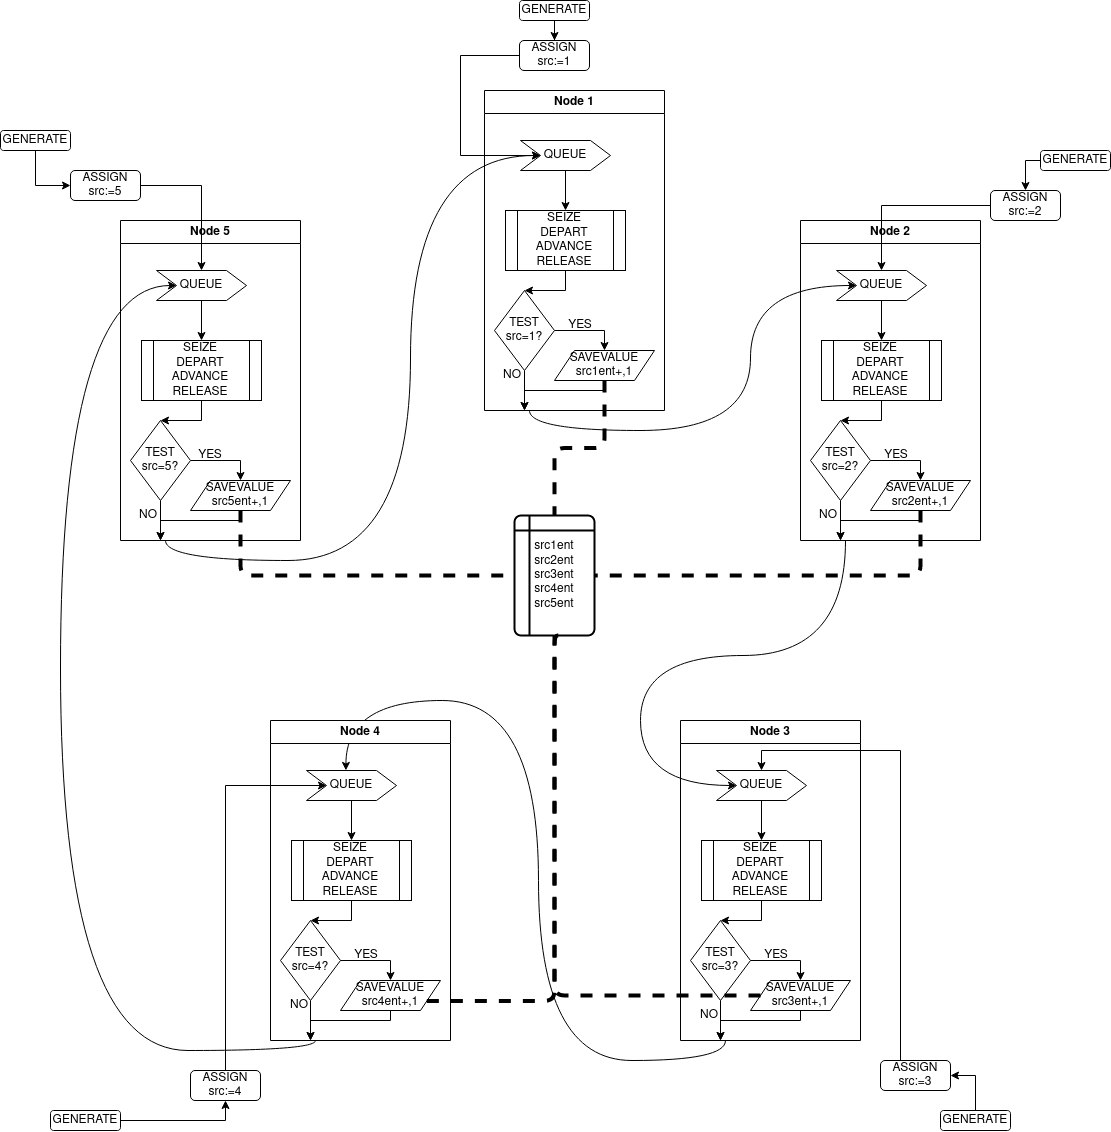
\includegraphics[width=\textwidth]{dia}

\section{Отчет}

Ниже приведен стандартный отчет GPSS World.
Согласно этому отчету, при $T=100000$, 
каждая заявка вернулась в исходный узел \textbf{4000 раз},
что указано в SAVEVALUE, связанных с ними.
Это значит, что одна заявка проходит цикл в среднем за \textbf{25 единиц времени},
потому что она проходит каждый элемент СМО в среднем за 5 единиц времени.
Поскольку утилизация каждого из FACILITY, связанных с элементами СМО, близка к 100\%,
из этого следует, что это значение соответствует настоящему пораметру системы.

\lstinputlisting[style=verbat]{lab2.report}


\end{document}